\documentclass{jfm}

\usepackage{xcolor}
\usepackage{array}
\usepackage{longtable}

\usepackage{graphicx,color}
% \usepackage[section]{placeins}
\usepackage{float}
% \usepackage{graphicx,subfigure}
\usepackage{subcaption}
\usepackage{epstopdf, epsfig}
\usepackage{amstext}
\usepackage{amsmath}
\usepackage{todonotes}
\usepackage{hyperref}
\usepackage{verbatim}
\usepackage{bm}
\usepackage{diagbox}
\usepackage{forloop}

\usepackage{listings}
\usepackage[numbered,framed]{matlab-prettifier}
% \let\ph\mlplaceholder % shorter macro
% \lstMakeShortInline"

\lstset{
  style              = Matlab-editor,
  basicstyle         = \mlttfamily,
  escapechar         = ",
  mlshowsectionrules = true,
}

\newtheorem{theorem}{Theorem}
\newtheorem{defn}{Definition}
\newtheorem{lemma}{Lemma}
\newtheorem{corollary}{Corollary}
\newtheorem{prop}{Proposition}
\newtheorem{assume}{Assumption}
\newtheorem{notation}{Notation}
\DeclareMathOperator*{\argmin}{arg\,min}

\newcommand\nc{\newcommand}
\nc\qu{\quad}
\nc\tends{\rightarrow}
\nc\dint{\int\!\int}
\newcommand{\vect}[1]{\mbox{\boldmath $#1$}}
\nc{\degree}{\mbox{\footnotesize{o}}}

\newcommand{\bes} {\begin{eqnarray*}}
\newcommand{\ees} {\end{eqnarray*}}
\newcommand{\dd} \partial

\newcommand{\non} \nonumber
\newcommand{\ie}{{\it i.e.}\ }
%\newcommand{\eg}{{\it e.g.}\ }
%\newcommand{\etal}{{\it et al.} \ }
\newcommand{\ru}{R_{\rm u}}
\newcommand{\rb}{R_{\rm b}}
\newcommand{\qup}{Q_{\rm u,pore}}
\newcommand{\qbp}{Q_{\rm b,pore}}

\newcommand{\ra}{\rightarrow}

\nc\cA{{\cal{A}}}
\nc\cB{{\cal{B}}}
\nc\cZ{{\cal{Z}}}
\nc\cX{{\cal{X}}}
\nc\cS{{\cal{S}}}
\nc\cR{{\cal{R}}}
\nc\cW{{\cal W}}
\nc\cU{{\cal U}}
\nc\cP{{\cal P}}
\nc\cF{{\cal{F}}}
\nc\cG{{\cal{G}}}
\nc\bz{\bar{z}}
\nc\bZ{\bar{Z}}
\nc\baz{\bar{\zeta}}
\nc\bw{\bar{w}}
\nc\bW{\bar{W}}
\nc\bX{\bar{X}}
\nc\bet{\bar{\eta}}
\nc\bp{\bar{\phi}}
\nc\bP{\bar{\Phi}}
\nc\bc{\bar{\chi}}
\nc\baf{\bar{f}}
\nc\baF{\bar{F}}
\nc\ov{\overline}
\nc\oW{\ov{W}}

\nc\hA{\hat{A}}
\nc\hB{\hat{B}}
\nc\ho{\hat{O}}
\nc\hG{\hat{\Gamma}}
\nc\hS{\hat{S}}
\nc\hO{\hat{\Omega}}
\nc\bO{\ov{\Omega}}
\nc\gham{\hat{\gamma}}
\nc\gcam{\check{\gamma}}
\nc\z{\zeta}
\nc\s{\sigma}
\nc\ep{\epsilon}
\nc\up{\upsilon}
\nc\lam{\lambda}
\nc\sig{\sigma}
\nc\om{\omega}
\nc\kap{\kappa}
\nc\gam{\gamma}
\nc\pa{\partial}
\nc\dom{\pa\Omega}
\nc\domt{\pa\tilde{\Omega}}
\nc\doh{\pa\hat{\Omega}}
\nc\pad[2]{\frac{\pa #1}{\pa #2}}
\nc\padd[2]{\frac{\pa^2 #1}{\pa {#2}^2}}
\nc\pard[3]{\frac{\pa^2 #1}{\pa {#2}\pa {#3}}}
\nc\nd[2]{\frac{d #1}{d #2}}
\nc\ndd[2]{\frac{d^2 #1}{d {#2}^2}}
\nc\ds{\displaystyle}
\nc\del{\nabla}
\nc\lap{\nabla^2}
\nc\ud{|\z|\leq 1}

\nc\capil{\mbox{Ca}}

\nc\pt{\tilde{a}}
\nc\ft{\tilde{f}}
\nc\vt{\tilde{v}}
\nc\wt{\tilde{w}}
\nc\nt{\tilde{\nu}}
\nc\xit{\tilde{\xi}}
\nc\xt{\tilde{x}}
\nc\etat{\tilde{\eta}}
\nc\nht{\tilde{\hat{\eta}}}
\nc\Taut{T}
\nc\zt{\tilde{\z}}
\nc\nut{\tilde{\nu}}

\nc\At{\tilde{\cA}}
\nc\qt{\tilde{B}}
\nc\Ct{\tilde{C}}
\nc\dt{\tilde{D}}
\nc\Dt{\tilde{\cU}}
\nc\Et{\tilde{L}}
\nc\Ft{\tilde{F}}
\nc\Ht{\tilde{H}}
\nc\Kt{\tilde{K}}
\nc\Lt{\tilde{K}}
\nc\Mt{\tilde{M}}
\nc\Nt{\tilde{N}}
\nc\Pt{\tilde{\Phi}}
\nc\Qt{\tilde{Q}}
\nc\Rt{\tilde{R}}
\nc\St{\tilde{\cS}}
\nc\Wt{\tilde{W}}
\nc\cWt{\tilde{\cW}}
\nc\Xt{\tilde{X}}

\nc\vs{\varsigma}
\nc\vp{\varpi}
\nc\ve{\varepsilon}
\nc\vepa{\ve_{\parallel}}
\nc\vepe{\ve_{\perp}}

%\bibliographystyle{elsarticle-num}


%\nc\captionsize{\footnotesize}

\newcommand{\pejman}[1]{\todo[inline,color=green!40]{Pejman: #1}}
\newcommand{\daniel}[1]{\todo[inline,color=yellow!40]{Daniel: #1}}
\newcommand{\michael}[1]{\todo[inline,color=red!40]{Michael: #1}}
\newcommand{\charles}[1]{\todo[inline,color=blue!40]{Charles: #1}}

\newcolumntype{A}[2]{%
    >{\minipage{\dimexpr#1\linewidth-2\tabcolsep-#2\arrayrulewidth\relax}\vspace\tabcolsep}%
    c<{\vspace\tabcolsep\endminipage}}

\newenvironment{lapsetable}[2]{ % n_cols, wid
    \tabular{
        cc
        *{#1}{>{\centering}A{#2}{1.5}}
    }
    \ignorespaces
    }{
    \tabularnewline
    \endtabular\ignorespacesafterend
}
\newenvironment{shortlapsetable}[2]{ % n_cols, wid
    \tabular{
        c
        *{#1}{>{\centering}A{#2}{1.5}}
    }
    \ignorespaces
    }{
    \tabularnewline
    \endtabular\ignorespacesafterend
}

\newcounter{lapse_iter}
\newcommand{\lapse}[9]{ % name, dt, N, dt_display, n_cols, *crop
    \tabularnewline
    #3 & #4
    \forloop{lapse_iter}{1}{\not{\value{lapse_iter} > #5}}{
        &
        \includegraphics[width=\textwidth, trim={#6cm #7cm #8cm #9cm}, clip]{tableFigs/#1/output_#2_#3/\arabic{lapse_iter}.pdf}
    }
}
\newcommand{\lapseShort}[6]{ % name, n_cols, width, *crop
    \forloop{lapse_iter}{1}{\not{\value{lapse_iter} > #2}}{
        &
        \includegraphics[width=\textwidth, trim={#3cm #4cm #5cm #6cm}, clip]{tableFigs/#1/\arabic{lapse_iter}.pdf}
    }
}
\newcommand{\scinote}[2]{{#1}$\times$10$^{#2}$}

\shorttitle{Droplets on a wall}
\shortauthor{M Li et al.}

\title{%Simulating a moving liquid-gas interface on an evolving solid surface with the extended Generalized Navier Boundary Condition through the immersed boundary Method
Simulating liquid-gas interfaces \\and moving contact lines \\with the immersed boundary method}
\author{Michael Y. Li$^{1}$, Daniel Chin$^{2}$, Charles Puelz\aff{3}, Pejman Sanaei\aff{4}\corresp{\email{psanaei@nyit.edu}}}
\affiliation{
    \aff{1}
    Courant Institute of Mathematical Sciences, New York University,\\ New York, NY 10012-1110, USA\\
    \aff{2}
    New York University Shanghai,\\ Shanghai, 200120, China\\
    \aff{3}
    Department of Pediatrics, Section of Cardiology, Texas Children's Hospital and Baylor College of Medicine, Houston, TX 77030-2372, USA\\
    \aff{4}
    Department of Mathematics, New York Institute of Technology,\\ New York, NY 10023-7692, USA\\
    $^{*}$M. Y. Li and D. Chin contributed equally to this work.
}

\begin{document}
\maketitle
\begin{abstract}
% In this work, we use the immersed boundary (IB) method to simulate the movement of 2D liquid droplets hanging on a vertical wall. The simulation requires moving contact line (MCL) and surface tension models that are built into the IB method. We propose an MCL model that enforces the Navier slip condition on the penalty-simulated immersed boundaries. The static and dynamic contact line angle are endogenous instead of prescribed. We use a liquid-gas interface model that is capable of simulating both a surface tension force and an unbalanced Young's force with one general equation that does not involve estimating local curvature. We also employ a step-wise re-sampling technique to ensure the uniform distribution of the Lagrangian markers that represent the liquid-gas interface and a step-wise interface splicing method to implement droplet coalescence and separation.

In this work, we propose and test four techniques that augments the immersed boundary method to simulate a moving liquid-gas interface on an solid surface. The first technique defines a moving contact line model and implements an extended Generalized Navier Boundary Condition at the immersed solid boundary. The static and dynamic contact line angles are endogenous instead of prescribed, and the solid boundary can be non-stationary with regard to time. The second technique simulates both a surface tension force and an unbalanced Young force with one general equation that does not involve estimating local curvature. The third technique splices liquid-gas interfaces to handle topological changes such as the coalescence and separation of liquid droplets or gas bubbles. The forth technique re-samples liquid-gas interface markers to ensure a near-uniform distribution without exerting artificial forces. We demonstrate empirical convergence of our methods and test them using some benchmark cases, including a slipping droplet on a wall and a rising bubble.
\end{abstract}

\begin{keywords}
% Authors should not enter keywords on the manuscript, as these must be chosen by the author during the online submission process and will then be added during the typesetting process (see http://journals.cambridge.org/data/\linebreak[3]relatedlink/jfm-\linebreak[3]keywords.pdf for the full list)
\end{keywords}

\section{Introduction}
Problems involving the coupling between a fluid and evolving immersed structures are usually impossible to describe analytically. The immersed boundary (IB) method is a numerical approach for solving such problems, traditionally with the assumption that the immersed boundaries are massless~\citep{peskin1972flow}. The method describes the fluid in Eulerian coordinates and the immersed boundaries with arrays of linked Lagrangian markers. The fluid advects the markers and the markers exert forces onto the fluid. The massless-boundary assumption is suitable for describing thin elastic membranes common in biological applications, for example, the interaction between blood flow and heart valves~\citep{peskin1972flow}. Similarly, the massless-boundaries assumption is appropriate for liquid-gas interfaces. Thus, with a surface tension model, the IB method is capable of modelling multi-phase fluid flow~\citep{leveque1997immersed, lorstad2004assessment, popinet2018numerical,  huang2018improved}. This bring a new challenge, which is the moving contact line (MCL) problem that emerges when a solid boundary meets with a liquid-gas interface. \citet{lai2010numerical} proposes an MCL model that simulates Navier slip with the IB method, but it is limited to \textit{fixed} solid boundaries. Note that, the Navier slip boundary condition in the wall of the moving contact line is used to avoid the force singularity~\citep{lai2010numerical}. 


In this work, we describe our MCL model that imposes an extended Generalized Navier Boundary Condition (GNBC)~\citep{quian2003generalized} between a moving liquid-gas interface and an \textit{evolving} immersed boundary. Two types of immersed boundaries (liquid-gas interface, solid surface) coexist and are governed by the same IB numerical method. The slip condition used in this paper is informed by recent molecular dynamics (MD) simulations \citep{johansson2018molecular}. The resulting numerical scheme, unlike related works that either prescribe the contact angle \citep{muradoglu2010front,liu2015diffuse} or specify the marker velocity \citep{manservisi2009variational}, is capable of capturing both the \textit{static} and the \textit{dynamic} contact angles in an endogenous way. 

In addition to the MCL model, we propose a surface tension model within the IB method. Using the IB method to simulate surface tension is often classified as a front-tracking scheme. Most front-tracking methods, including many IB variants, calculate the magnitude of surface tension by estimating the local curvature of the interface using three to six markers~\citep{leveque1997immersed, huang2018improved}. This approach is susceptible to errors and instability issues. \citet{tryggvason2001front} computes the surface tension using tangent vector subtraction in every Eulerian cell, thus omitting the need to estimate curvature. \citet{popinet1999front} uses tangent vector subtraction for every link between adjacent Lagrangian markers, exploiting the IB method's Lagrangian representation of the structure. Our method uses tangent vector summation for every Lagrangian marker (instead of every link). The subtle shift in perspective brings a side benefit that the unbalanced Young force \citep{quian2003generalized} at the contact point is readily computed by the two markers at both ends of a liquid-gas interface. In addition, our approach uses a step-wise re-sampling technique to ensure a near-uniform distribution of Lagrangian markers in the liquid-gas interface. Finally, we employ a step-wise interface splicing method to implement interface topological changes including droplet coalescence and separation. 

This study is motivated by a real-life industerial problem~\citep{MPIreport2018}, presented by W.L.~Gore \& Associates. Catalysts are an integral part of many chemical processes. They are usually made of a dense but porous material such as activated carbon or zeolites, which provides a large surface area. Liquids that are produced as a byproduct of a gas reaction at the catalyst site are transported to the surface of the porous material, slowing down transport of the gaseous reactants to the catalyst active site. One example of this is in a sulphur dioxide filter, which converts gaseous sulphur dioxide to liquid sulphuric acid. Such filters are used in power plants to remove the harmful sulphur dioxide that would otherwise contribute to acid rain. Understanding the dynamics of the liquid droplets in the gas channel in a device is critical in order to maintain performance and durability of the catalyst assembly. %This scenario is based on a real-life case where a vertical catalyst scaffold removes pollutants such as sulfur dioxide from industrial exhaust before release into the atmosphere, which is of considerable environmental interest \citep{MPIreport2018}.
Among several other tests, our methods presented in this paper are applied to simulate 2D droplets moving on a vertical wall. In this paper, we empirically study the spatial and temporal convergence of our methods, compare simulation results at equilibrium against an analytical solution, and benchmark our methods with several standard test cases.

The paper is organized as follows: in \S\ref{sec:numerical} we describe the IB method, the boundary conditions, the surface tension formulation, the moving contact line problem, the step-wise interface re-sampling technique, and the interface splicing technique. An approach for simulating a variable fluid density is also discussed. We then introduce the discretization of the governing equations in \S\ref{sec:discretization}. In \S\ref{sec:tests}, we present our simulation results. Finally, we conclude in \S\ref{sec:conclusion} with a discussion of our model and results, and we provide some insight into real-world applications.

\section{Equations of motion} \label{sec:numerical}
In this section, we describe the IB method. This approach has proven to be an extremely versatile method for fluid-structure interaction problems since its development almost forty years ago~\citep{peskin1972flow,mcqueen1997shared,arthurs1998modelling,lai2000immersed,griffith2009simulating,balboa2011staggered,devendran2012immersed,sanaei2021flight}. The method represents the immersed structure with Lagrangian coordinates and the fluid with Eulerian or `lab frame' coordinates. The interactions between the two coordinate frames are communicated with integral transforms involving Dirac delta function kernels. For the solid surfaces considered in this paper, we adopt the penalty immersed boundary (pIB) method \citep{kim2016penalty}, which introduces a set of \textit{tether points} that are fixed in space and represent the desired shape and location of the structure. The boundary markers are connected to the tether points via springs, and only the boundary markers interact with the fluid. Stiff springs approximate a rigid boundary. These stiff springs result in numerical stiffness but simplify the implementation. In practice, accurate results can be achieved with an appropriate choice of the spring constant, spatial discretization, time stepping, and other numerical parameters \citep{kim2016penalty}. 

The equations of motion for the coupled fluid-structure system are:
\begin{align}
\rho\left(\cfrac{\partial\bm{u}}{\partial t}+\bm{u}\,\nabla\bm{u}\right) & =
    -\nabla p+\mu\Delta\bm{u}+\bm{f}_1+\bm{f}_2+\bm{f}_3,
    \quad
    \nabla \bm{u}=0, \label{eq:ib-ns} \\
\bm{f}_i(\bm{x},t) & = 
    \begin{cases}
    \int  \bm{F}_i(   s,t)\,\delta(\bm{x}-\bm{X}_i(   s,t))\,ds,     \quad &i = 1,2, \\ \\
    \iint \bm{F}_i(r, s,t)\,\delta(\bm{x}-\bm{X}_i(r, s,t))\,ds\,dr, \quad &i = 3, 
    \end{cases}
    \label{eq:ib-spread-force} \\
\cfrac{\partial\bm{X}_i}{\partial t}(t) &=
    \int\bm{u}(\bm{x},t)\,\delta(\bm{x}-\bm{X}_i(t)) \, d\bm{x}, \quad i = 1,2,3.
    \label{eq:ib-advect}
\end{align}

Here $\rho$ and $\mu$ are the density and dynamic viscosity of the fluid. $\boldsymbol{u}(\boldsymbol{x},t)$ is the velocity and $\delta$ is the 2D Dirac delta function. $\boldsymbol{x}$ and $\boldsymbol{X}_i$ denote the Eulerian fluid coordinates and the Lagrangian structure coordinates. In this paper, we consider three types of immersed structures: a 1D wall boundary ($\bm{X}_1$), a 1D fluid-gas interface boundary ($\bm{X}_2$), and a 2D variable density area ($\bm{X}_3$). With the 1D structures, $s$ is the arc length that specifies a point on the boundary (i.e. an arc length-conserved parametrization of the 1D boundary). With the 2D structures, $(r,s)$ is a 2D equidistant parametrization of the area. $\boldsymbol{f}_i$ and $\boldsymbol{F}_i$ are the Eulerian and the Lagrangian force densities corresponding to the immersed structures. The Lagrangian force densities $\boldsymbol{F}_1$ and $\boldsymbol{F}_2$ are 1D force densities but $\boldsymbol{F}_3$ is a 2D force density. The following subsections will introduce each type of immersed structure $\boldsymbol{X}_i$ and define its force densities $\boldsymbol{F}_i$. Formulas  (\ref{eq:ib-ns}) are the Navier-Stokes equations for incompressible flow of a viscous fluid. Equation (\ref{eq:ib-spread-force}) describes how force is imparted from the immersed structures to the fluid by defining the Eulerian force density. Note that the Dirac delta function kernel converts the Lagrangian force density $\bm{F}_i$ to the corresponding Eulerian force density $\bm{f}_i$. Equation (\ref{eq:ib-advect}) ensures the velocity of the immersed structures is the same as the fluid velocity, i.e. no-slip and no-penetration condition between the fluid and structure. 



\subsection {Boundary conditions} \label{sec:bc}
\begin{figure}
\centering
\includegraphics[scale=0.35]{figs/domain_schematics/domain.pdf}
\caption{\footnotesize The underlying computational domain exposed to the fluid solver is 2 cm $\times$ 2 cm. The effective boundary conditions for the 1 cm $\times$ 2 cm problem domain are shown via parenthesized texts. The effective symmetry boundary is obtained by mirroring half of the simulation domain. The GNBC is obtained by adding a wall (see \S\ref{subsec:wall}) at the periodic boundary.}
\label{fig:domain}
\end{figure}
The Matlab implementation of IB by \citet{ib_matlab} prescribes the periodic boundary condition for the computational domain. In most of our simulations, we fold the domain in half to obtain a symmetry boundary condition on the left and right boundaries. This section describes our implementation of symmetry boundary conditions within Peskin's implementation. 

If $L \times L$ is the computational domain in $(x,y)$ exposed to the fluid solver (figure ~\ref{fig:domain}), then we select the left half of it, $L/2 \times L$, to be the problem domain. According to figure ~\ref{fig:domain}, $L=2$ is chosen. During each time step, once the Eulerian force densities (given by equation \ref{eq:ib-spread-force}) are imparted onto the grid, the simulation mirrors the Eulerian force densities matrix around $x = L/2$ (i.e. the dashed line in figure ~\ref{fig:domain}) and add it back to the original Eulerian force field. In this way, the fluid velocity field is always symmetric around $x = L/2$. In other words, we `waste' the right half of the computational domain in order to prescribe the symmetry boundary condition on the left half. 

% \charles{the following sentences discussing indexing are probably not necessary.}
% The specific indexing of the 2D force densities matrix with \citet{ib_matlab}'s code involves extra complexity since the Eulerian coordinates $(0, 0)$ maps to matrix location $(1, 1)$. This means the axis of symmetry, in terms of matrix indices, is $N / 2 + 1$. Therefore, matrix location $(N / 2 - i, j)$ is in symmetry with matrix location $(N / 2 + 2 + i, j)$ for integer $i, j$. 

\subsection{Wall as an immersed boundary} \label{subsec:wall}
The main case that motivates our study is the simulation of liquid droplets moving on a solid vertical wall. We simulate the wall as an immersed boundary. In this specific case, since the wall is static, it is arguably easier to treat the wall as a boundary condition. However, we want our MCL method to generalize to non-static solid surfaces (see e.g. \S\ref{subsubsec:letters}), so we treat the wall as an immersed boundary to maximize generality. Each Lagrangian marker of the wall is tethered to its ground-truth location, thus ensuring no penetration and no slip, therefore he Lagrangian force density corresponding to the 1D wall is
\begin{equation}
\bm{F}_1(s,t) = -k_1 \, (
    \bm{X}_1(s,t) - \bm{Z}(s)
). 
\label{eq:wall-force}
\end{equation}
Equation (\ref{eq:wall-force}) describes the tether-point construction and the associated spring force on the boundary to model a no-slip and no-penetration wall. The parameter $k_1$ is the spring constant ($\text{g}/(\text{s}^2\,\text{cm}$)) associated with the wall, which is a trade-off parameter between accuracy and numerical stability. $\boldsymbol{Z}$ is the ground-truth location. At the start of the simulation, we usually initialize $\boldsymbol{X_1}(s,0) = \boldsymbol{Z}(s)$ (with \S\ref{subsec:rb} as an exception). The wall behaviour will be later modified in the MCL model, as described in \S\ref{subsec:mcl}. 

\subsection{Surface tension}
We use the integral formulation as described by \citet{popinet2018numerical} to derive a model for surface tension. In this approach, each interface marker is pulled by its two neighbours at a constant magnitude. In contrast to \citep{tryggvason2001front}, our method is entirely in the Lagrangian frame and does not estimate a tangent vector with a polynomial fit. Instead, the unit tangent vector is 
\begin{equation}
\bm{\hat{T}}(s, t) = \cfrac{\partial \bm{X}_2(s, t)}{\partial s}. 
\end{equation}
Then, the Lagrangian surface tension force density is
\begin{equation}
\bm{F}_2(s,t) = \sigma \cfrac{\partial \bm{\hat{T}}}{\partial s}. 
\end{equation}
where $\sigma$ is the surface tension coefficient. 
Therefore, for a segment $AB$ of the interface as shown in figure ~\ref{fig:integralFormulation}, we have
\begin{equation}
\int_{\Omega} \bm{F}_2 \, ds = \int_{A}^{B} \sigma \, d \bm{\hat{T}} = \sigma (\bm{\hat{T}}_B - \bm{\hat{T}}_A),
\end{equation}
 \label{eq:tension}
\begin{figure}
    \centering
    \includegraphics[width=7cm]{figs/integralFormulation.pdf}
    \caption{\label{fig:integralFormulation}
        An interface marker $X_{\ell_0}$ is responsible for the surface tension force on the red segment $AB$. $\bm{\hat{T}}_A$ (the unit tangent vector at $A$) is computed by subtracting the marker $X_{\ell_0}$ from the adjacent marker $X_{\ell_0-1}$. The difference between $\bm{\hat{T}}_A$ and $\bm{\hat{T}}_B$ (the unit tangent vector at $B$), multiplied by the tension coefficient $\sigma$, gives the surface tension force on the segment $AB$. $\Omega$ is the set of interface parametrization $s$ on segment $AB$. This is then numerically applied to point $X_{\ell_0}$. 
    }
\end{figure}
where $\bm{\hat{T}}_A$ and $\bm{\hat{T}}_B$ are the unit tangent vector at $A$ and $B$, respectively. With this approach, the sum of surface tension forces in a closed loop is zero \citep{popinet2018numerical}. In our discrete implementation as shown in figure ~\ref{fig:integralFormulation}, we first compute the tangent vectors pointing from one marker to its adjacent markers and then apply the corresponding force, of magnitude $\sigma$, onto the marker. 

\begin{figure}
    \centering
    \includegraphics[width=5cm]{figs/young.pdf}
    \caption{\label{fig:young}
        The blue circles show the interface markers. The surface tension force is applied in the tangent direction $\bm{\hat{T}}$ from every marker to its two adjacent markers. This scheme leaves the two markers at the wall with only one adjacent marker, simulating the unbalanced Young force with the same method as the tension force. Notice that the sum of the tension forces on all markers is exactly the sum of unbalanced Young forces on the two markers, just inverted in direction. 
    }
\end{figure}
A consequence of this implementation is that when the gas-liquid interface meets a solid surface, the unbalanced Young force~\citep{quian2003generalized}, denoted by $\bm{f}_Y$, becomes a side benefit of surface tension and is correctly imparted. As shown in figure ~\ref{fig:young}, at a contact point, there is one interface marker that only has one neighbour. The total force on this marker becomes tangent, instead of normal, to the interface. The horizontal component of this force is balanced by the tether force provided by the no-penetration wall, and the vertical component is the unbalanced Young force, 
\begin{equation}
    \bm{f}_Y = \bm{\hat{T}} \, \sigma \cos\theta. \label{eq:young}
\end{equation}
where $\theta$ is the contact angle. To re-iterate, our numerical simulation never uses the above formulation of $\bm{f}_Y$ since the unbalanced Young force is already included in our surface tension implementation. 

\subsection{Moving contact line and the extended Generalized Navier Boundary Condition} \label{subsec:mcl}
The MCL problem refers to the apparent contradiction that contact lines can move on a no-slip wall. The mechanism of an MCL and how to simulate it had been largely a mystery until 1979~\citep{dussan1979spreading}. Since then, researchers have developed many numerical models of MCL \citep{sui2014numerical, liu2015diffuse}. A recent study by \citet{johansson2015water} discovered that hydrogen bonds facilitate the no-slip behaviour of water on hydrophilic surfaces. These bonds are orders of magnitudes stronger compared to the fluid's internal viscosity, so hydrophilic surfaces usually behave as if they were no-slip. That justifies the traditional no-slip assumption between water and hydrophilic surfaces. MCL breaks that assumption as the unbalanced Young stress at the contact point breaks the hydrogen bonds, therefore allowing slip. The energy dissipation from slipping has been quantified by molecular dynamics (MD) simulations~\citep{johansson2018molecular}. In conclusion, where there is an MCL, it is proper to allow slip at the wall. For example, in~\citep{lai2010numerical}, MCL is simulated with IB by implementing a GNBC in the fluid solver. However, if the geometry of the solid boundary evolves with time, imposing it onto the fluid is still challenging. This section proposes a method to implement an extended GNBC on an evolving immersed boundary. 

With a GNBC, the slip velocity is proportional to the sum of the tangential viscous stress and the unbalanced Young stress. Coincidentally, as the IB method sums up the Eulerian force densities imparted from different types of boundaries, the local total tangential stress becomes readily available, so we have no need to distinguish the unbalanced Young stress from the internal viscous stress. In this light, we propose a wall friction model that is analogous to the viscous force within the fluid. \charles{why is a frictional model similar (the same) as GNBC?} In this analogy, the viscous force is the friction between adjacent layers of the fluid, while the wall friction is the friction between the wall and the first layer of the fluid. Using a linear friction model results in equations of motion identical to the GNBC. For example, when the unbalanced Young stress exactly cancels the friction force, the slip velocity will be constant, and the friction force will be proportional to the slip velocity. Moreover, we extend the GNBC so that weak tangential stress results in a stationary contact. Specifically,
\begin{align}
\bm{F}_t & = \left( \bm{F}_1 \cdot \bm{\hat{t}} \right) \, \bm{\hat{t}}, \\
\bm{F}_f & = \min \{ \lVert \bm{F}_t \rVert, F_\text{static limit} \}
\left(
- \cfrac {\bm{F}_t} {\lVert \bm{F}_t \rVert}
\right), \\
F_\text{static limit} & =
F_\text{no-slip} + \eta(\theta)
\left|
    \bm{u} \cdot \bm{\hat{t}}
\right|, 
\label{eq:friction}
\end{align}
where $\bm{F}_f$ is the resulting wall friction density (1D), $F_\text{static limit}$ is the static stress threshold, $\bm{F}_t$ is the local tangential stress, $F_\text{no-slip}$ is the minimum friction density (discussed below), $\theta$ is the contact angle, $\eta$ is a mapping from a contact angle to a friction coefficient (cm$^{-1}$), and $\bm{\hat{t}}$ is the unit vector tangent to the wall. Note that $\bm{F}_t$ is computed from the wall marker tether force density $\bm{F}_1$ which is the way that IB captures the instantaneous local stress. 

The function $\eta$ gives the friction coefficient (cm$^{-1}$) from the contact angle $\theta$ and is defined as:
% \charles{I might put the function below in an appendix. where do the numbers come from?  might want to cite the paper in the listing caption. we might also want a LaTeX'ed $\mu(\theta)$ function directly in the text if it is possible to do so.}  
\begin{equation}
\eta(\theta) = %\text{cm}^{-1} \cdot
\begin{cases}
    1.54 & \text{if   }\ \theta > 2, \\
    - 8.48\,\theta + 18.5 & \text{if   }\ 1.117 < \theta \le 2, \\
    - 19.1\,\theta + 30.31 & \text{if   }\ \theta \le 1.117. 
\end{cases}
\end{equation}
Those numbers (e.g. $1.54$, $8.48$, etc.) in the friction coefficient $\eta$ are based on measured results from a simulation of water-silica contact line movement by \citet{johansson2018molecular}. Linear interpolation of measured data points is used to fill the continuous domain of $\theta$. Notice that our MCL method is agnostic to the specific implementation of $\eta$, therefore future usages are free to modify $\eta$. 
% We believe more accurate simulation results can be obtained by fine-tuning $\eta$ based on MD studies such as~\citep{qian2004power}. 

%We now take a closer look at the behaviours governed by equation \ref{eq:friction}. 
Note that, according to (\ref{eq:friction}), when the contact angle is very large and the unbalanced Young force becomes weak such that $\|\bm{F}_t\| < F_\text{static limit}$, then we have $\bm{F}_f = -\bm{F}_t$ where the wall behaves as if it was governed by the no-slip condition. This is what sets our method apart from the (non-extended) GNBC: with GNBC, any non-zero tangential stress, no matter how weak, moves the contact line. Our extended GNBC allows no slip under sufficiently weak tangential stress, which better describes the physical reality. Additionally, the GNBC becomes a special case of the extended GNBC where $F_\text{no-slip} = 0$. 
\daniel{check above paragraph for language}

% The last prerequisite concept we need to introduce is the \text{slip length}, $l$. $l$ has the unit cm and describes the length of the local region that affects slipping. In IB, slipping

Finally, this frictional force is incorporated into the IB method by making the wall markers' tether force $\bm{F}_1$ equal to $\bm{F}_f$. To do this, at every time step, each wall marker is tangentially displaced until the tangential component of the tether force becomes equal to $\bm{F}_f$ (see figure ~\ref{fig:displace}). The ground-truth locations $\bm{Z}$ is unchanged, and (\ref{eq:wall-force}) which computes $\bm{F}_1$ still holds. The displacement can be viewed as a modification to the advection equation (\ref{eq:ib-advect}). We emphasize three outcomes from this rule: 
% \charles{the frictional implementation is not clear to me.  do you have markers for the wall and markers for the the droplet at the wall?  do you only exert the frictional force on one of these sets of markers? }\daniel{the friction force is the tether spring force, so it is exerted onto the wall.}
\charles{consistent notation and terminology should be used here, i.e. the frictional force should really be a formula for $\bm{F}_1$, correct? what is that formula, and what happens with the ground-truth locations $\bm{Z}$ for the wall?}
\begin{itemize}
    \item The contact line can now slip. Slipping is the accumulation of the tangential displacement of wall markers. 
    \item The resistive force (i.e. tether force) that the wall exerts onto the fluid equals the above-formulated $\bm{F}_f$. 
    \item The work done by the friction, i.e. heat dissipation, is accurately removed from the system, as the tangential displacement of wall markers consumes some potential energy in the tether springs. 
    \item $\bm{F}_f$ can be viewed as the no-slip version of $\bm{F}_1$ with an upper bound of $F_\text{static limit}$. When bounding, wall markers get displaced, and slip happens. In contrast, the no-slip baseline (\S\ref{subsec:wall}) imposes no upper bound. The tangential stress, no matter how strong, is matched by the resistive force provided by the wall, so there is no slip. 
    \item The resulting macroscopic behaviours of extended GNBC are analogous to how rigid bodies display static and sliding frictions. If $F_\text{static limit}$ is bounding, we have sliding friction (slip), otherwise we have static friction (no-slip). 
\end{itemize}
The numerical implementation involves a trivial algorithm that associates each wall contact with a local region of the wall, so that the contact line velocity is available for calculating the friction force. 
\begin{figure}
    \centering
    \includegraphics[width=4.5cm]{figs/displace.pdf}
    \caption{
        Tangential (in this case, vertical) displacement of the marker constitutes slip. There is never any normal (in this case, horizontal) displacement, ensuring no penetration. 
    }
    \label{fig:displace}
\end{figure}

\subsection{Step-wise interface re-sampling}
The surface tension is always normal to the interface, therefore, the fluid flow easily disrupts the distribution of the interface markers. To equi-distribute the markers on the structure,~\citet{lai2008immersed} used grid redistribution, while \citet{hou1994removing, lai2010numerical} applied artificial tangential velocity. Our method is similar to grid redistribution in the sense that we add markers to wide gaps and remove them from tight spaces at every time step. Specifically, at each time step, the program iterates over all the interface markers. When the distance between any pair of markers exceeds $\sqrt{2}$ times their initial distance, the program inserts a new marker between them. When the distance between the outer two of any three adjacent markers become smaller than $\sqrt{2}/2$ times their initial distance, the program removes the inner marker of the three. 

Whenever a marker is removed, the two adjacent markers are joined together and their coordinates are left untouched. However, a \textit{sharpness check} compares $\cos \alpha$ (where $\alpha$ is the angle formed by the three markers) with a threshold ($0.9$, in our case) to prevent the program from removing a marker that represents a relatively sharp corner and adversely affecting area and tension energy conservation. The sharpness check becomes irrelevant as the spatial discretization resolution $N$ approaches infinity but improves simulation accuracy for finite values of $N$. 

\begin{figure}
    \centering
    \includegraphics[width=9cm]{figs/addMarker.pdf}
    \caption{
        The blue circles show four adjacent interface markers. When the distance between the inner two is larger than $\sqrt{2}$ times its initial length, we insert a new marker. IX is the intersection of two lines, one connecting $X_{\ell_0-1}$ to $X_{\ell_0}$ and the other connecting $X_{\ell_0+2}$ to $X_{\ell_0+1}$. MP is the midpoint of the line segment between $X_{\ell_0}$ and $X_{\ell_0+1}$. The green cross shows the location to add the new marker at, which is a linear combination of MP and IX weighted by an amendment factor. 
    }
    \label{fig:add-marker}
\end{figure}
On the other hand, when a marker is inserted (figure ~\ref{fig:add-marker}), the program calculates two locations: the midpoint (MP) between the two markers and the intersection (IX) of the extrapolated lines from four adjacent markers. A weighted average between MP and IX is used as the location for the newly inserted marker. The averaging is weighted by a \textit{re-sampling amendment factor}. If there is too much weight on the midpoint, the removal of markers will erroneously decrease tension energy while insertion will not increase tension energy. By having a proper weight on the extrapolated intersection, we can keep the \textit{bias} of the energy error to $0$ (although the \textit{variance} will still increase with time). On the other hand, too much weight on the extrapolated intersection leads to alternating jagged edges and eventually to instabilities. In our simulations, we set the re-sampling amendment factor to be $0.5$. The amendment factor becomes irrelevant as $N$ approaches infinity but improves simulation accuracy for finite values of $N$.

Our re-sampling routine constantly computes and records energy errors due to the artificial removal and insertion of markers. At the end of a simulation, these errors can be plotted for evaluation. See \S\ref{subsec:resample} for the apparent improvement that this technique brings. This re-sampling technique, however, is very difficult to extend to 3D with a surface mesh.  

\subsection{Interface splicing} \label{subsec:splice}
\begin{figure}
\centering
\subfloat[]{\includegraphics[scale=0.2]{figs/splice.pdf}}\quad
\subfloat[]{\includegraphics[scale=0.32]{figs/splice_case.pdf}}\\
\caption{\footnotesize (a): Among the six interface splicing scenarios, three pairs are reversed in time and three pairs share the same implementation. (b): An important condition for splicing to happen is that the two interfaces are approaching, as shown with the violet arrows representing velocity of each interface. When the distance between four involved markers become small enough, the algorithm splices the interfaces (removing two black links and adding two green links).}
\label{fig:splice}
\end{figure}
figure ~\ref{fig:splice}(a) shows six possible scenarios in which the liquid-gas interface changes topology and the chain of interface markers needs to be spliced: two droplets merging, one droplet splitting into two, a droplet attaching to the wall, a droplet detaching from the wall, a droplet splitting at the wall, and droplets merging at the wall. Those six cases form three pairs of reversed processes as well as three pairs of scenarios whose implementations are exactly the same. The same-implementation cases are locally indistinguishable, since our splicing implementation is agnostic to the phase (i.e. whether liquid or gas) on each side. 

To implement splicing, we store the interface markers in circular double linked lists. The linking direction preserves the polarity information: if one follows the links in the positive direction, the liquid will always be on the right. figure ~\ref{fig:splice}(b) illustrates a splicing event. When the distance between two interfaces is smaller than a threshold, the simulation further checks whether the two interfaces are approaching using the sign of the dot product of their velocities. If both conditions hold true, the interfaces are spliced together. In our method, we have two different distance thresholds, one for interface-interface events ($h$), and the other for interface-wall events ($2.3h$), where $h$ is the meshwidth (i.e. diameter of one Eulerian grid cell). These specific parameters result in stable splicing events according to our subjective experiences with demo runs. 
% These thresholds will be further optimized in future work. 

% \charles{sentence below does not make sense}
A splicing event make the two subsequent time steps skip the splicing subroutine. This rule makes splicing events more atomic so that there will not be multiple splicing events competing to accomplish the same macroscopic effect. 

\subsection{Variable density}
Our model uses the technique proposed by \citet{kim2008numerical} to describe the different densities for the liquid within the droplet and the gas outside of the droplet. In this approach, a 2D grid of Lagrangian markers are uniformly spawned in the liquid phase to represent density differences. These markers have an effective mass because they are tethered to their massive, Newtonian counterparts using the penalty immersed boundary (pIB) method. More formally, the Newtonian particles have velocity $\boldsymbol{v}$, 
\begin{equation}
\bm{v}(s,r,t) = \cfrac{\partial \bm{Y}(s,r,t)}{\partial t}.
\end{equation}
where $\boldsymbol{Y}$ is the location of the Newtonian particles. 
The forces on the Newtonian particles are the tether force and the gravity: 
\begin{equation}
\Delta \rho \, \cfrac{\partial \bm{v}(s,r,t)}{\partial t} = k_3 \, (
    \bm{X}_3(s,r,t) - \bm{Y}(s,r,t)
) - \Delta \rho \, G \, \bm{\hat{j}},
\end{equation}
where $\Delta \rho = \rho_\text{liquid} - \rho_\text{gas}$ is the density difference, $G$ is the gravitational constant, and $k_3$ is the spring constant ($\text{g}/(\text{s}^2\,\text{cm}^2)$) associated with the variable density method. Finally, the tether force is applied as a force density onto the fluid:
\begin{equation}
\bm{F}_3(s,r,t) = k_3 \, (
    \bm{Y}(s,r,t) - \bm{X}_3(s,r,t)
). 
\end{equation}

In our simulation we use the variable density method~\citep{kim2008numerical} with some modifications. \citet{kim2008numerical} used a five-step update method for time stepping, while we use a coarser, midpoint method (see \S\ref{sec:discretization}). We also set the \textit{allowed distance}\footnote{The \textit{allowed distance} is a parameter in the method by \citet{kim2008numerical}. It sets a ceiling for the distance between a boundary marker and its Newtonian counterpart. In our studies, the program monitors the maximum distance between a boundary marker and its Newtonian counterpart. Once it exceeds the allowed distance, the program raises a warning for the human conductor to increase the pIB spring stiffness and rerun the simulation.} to be one tenth the mesh-width, $h/10$. 

%\section{Scaling \& nondimensionalization} \label{sec:scaling}
\section {Numerical discretization\label{sec:discretization}}
% \michael{... and the subscript of the delta function should be $h$ instead. I commented some of the scripts you wrote and add my version.}
% \daniel{COuld you go ahead and change the subscript of delta, if you are sure?}

For the spatial discretization, we use a global Navier-Stokes solver based on harmonics in the velocity field. This solver uses the Fast Fourier Transform to accelerate the computation, but at the cost of not being able to handle variable density/viscosity out-of-the-box. The time step is denoted $dt$ with units of seconds. The spatial discretization parameter, denoted $N$, is the number of Eulerian cells in the problem domain along the $y$ axis. The length of the side of a cell in the spatial discretization, i.e. the meshwidth, is denoted $h$ with units of centimeters. Therefore, we always have $N \, h = L$ where $L$ is the height of the problem domain. 

The time step index is denoted $n \in \{0, 1, 2, ...\}$. The physical time at time step $n$ is given by $t^n = n \, dt$. The discrete, Eulerian space coordinates that label the cells in the Cartesian mesh are $(i, j) \in \{0, 1, 2, ..., N-1\}^2$. A physical cell position in the problem domain is given by ${\bm x}_{ij} = (i \, h, j \, h)$,
where the meshwidth $h = L / N$. The fluid velocity  $\boldsymbol{u}(x_{ij},t^n)$ at position $x_{ij}$ and time $t^n$ is approximated by the discrete fluid velocity represented as $\bm{u}_{ij}^n$, and the array of discrete velocities at time step $n$ is denoted ${\bm u}^n = (\bm{u}_{ij}^n)$. %like this: 
% \begin{equation}
% \bm{u}_h^n(\bm{x}_{ij}). 
% \end{equation}
The discrete spatial parametrization variables for the immersed structures are $\ell \in \{0, 1, 2, ..., \ell_{max}\}$ and $m \in \{0, 1, 2, ..., m_{max}\}$ where $\ell_{max}, m_{max}$ can change during simulation because of interface re-sampling. A point within the parametrization of the immersed structure is given by $(r_\ell, s_m) = (\ell \, \Delta r, m \, \Delta s)$ where $\Delta r, \Delta s$ control the discrete spatial resolution of the structures. In our simulations, we initialize $\ell_{max}$ and $m_{max}$ so that $\Delta r = \Delta s = h / 2$. The discrete 2D structure positions corresponding to the variable density area $\bm{X}_3$ are indexed as  $\bm{X}_{\ell m}^n \approx \bm{X}(r_\ell,s_m,t^n)$. We use the same notation for the 1D wall boundary $\bm{X}_1$ and the 1D fluid-gas interface boundary $\bm{X}_2$ for simplicity, although in these cases there is only a single parametrization variable. The array of discrete structure positions at time step $n$ is denoted $\bm{X}^n = (\bm{X}_{\ell m}^n)$.

% \charles{The discretization of the independent variables should be put before the discussion of the discrete velocity and structure positions.}

% time step n; parenthesis refers to space. 
We use a \textit{midpoint method} for evolving the system in time that relies on quantities at intermediate time steps $\{\frac{1}{2}, \frac{3}{2}, ...\}$. This method has the effect of improving stability and constraining numerical errors. Following the approach from~\citep{peskin2002immersed, ib_matlab} the procedure below is a time discretization of the equations of motion (\ref{eq:ib-ns}), (\ref{eq:ib-spread-force}), and (\ref{eq:ib-advect}): 
\begin{enumerate}
    \item Given the marker positions $\bm{X}^n$ and the fluid velocity $\bm{u}^n$, compute the first-order approximation of marker positions at the midpoint step $\bm{X}^{n + 1/2}$. 
    \item Given the marker positions at the midpoint step $\bm{X}^{n + 1/2}$, compute the force densities at the midpoint, denoted $\bm{f}^{n + 1/2}$. \footnote{Spreading Lagrangian force density $F_h$ to Eulerian force density $f_h$ uses the discrete 2D Dirac delta function \citep{peskin2002immersed}.}
    \item Given the fluid velocity field $\bm{u}^n$ and the force densities at the midpoint step $\bm{f}^{n + 1/2}$, compute the fluid velocity field at both the midpoint $\bm{u}^{n + 1/2}$ and the next time step $\bm{u}^{n + 1}$. 
    \item Given the marker positions $\bm{X}^n$ and the fluid velocity at the midpoint step $\bm{u}^{n + 1/2}$, advect the markers for $dt$ to obtain the marker positions at the next time step $\bm{X}^{n + 1}$. 
\end{enumerate}
\section {Test cases and results\label{sec:tests}}
In this section, we describe the application of our numerical techniques to simulate several test cases. In \S\ref{subsec:equi}, we simulate a hanging droplet on a wall and compare our results to the equilibrium state with an analytical solution. In \S\ref{subsec:rb}, we compare our simulation with an established benchmark in which a bubble rises in a liquid column. In \S\ref{subsec:dow}, we describe results from various test cases in which a droplet slides down a wall. Convergence tests for our method, with respect to the time step and spatial discretization, are shown in \S\ref{subsec:converg}. Some cases involve droplet coalescence and separation. In \S\ref{subsec:resample} we explore the importance of our interface re-sampling technique. Finally, in \S\ref{subsec:more_splice}, we showcase some additional tests in which interfaces are spliced to represent topological changes. 

We urge the reader to check out the simulation videos at ...
\daniel{remember to add videos}

\subsection {Comparison with an analytical solution in hydro-static equilibrium}\label{subsec:equi}
In this test, we compare our simulation results with an analytical solution for the interface shape of a droplet hanging on a vertical wall in hydro-static equilibrium. Details regarding the analytical solution are given in Appendix~\ref{app:equi}. 

For these simulations, the time step is $dt=0.0001$ s, the spatial discretization parameter is $N=96$, the height of the computational domain is $L=2$ cm, the tension coefficient is $\sigma=100$ g\,cm/s$^2$, the gas density is $\rho_g=0.1$ g/cm$^2$, the liquid density is $\rho_l=1$ g/cm$^2$, and the viscosity is $\mu=1$ g/s. We run several simulations and vary the magnitude of gravity coefficient $G$ to compare curvatures in the equilibrium state against the analytical solution. To estimate local curvature at each marker, we compute the circle that contains the three adjacent markers and calculate the inverse of the circle's signed radius. The simulations are terminated at $t = 0.25$ s, at which time all three cases have reached a steady state. Results are shown in figure ~\ref{fig:h-curvature}. A linear relation is seen between the 2D curvature and the altitude. As shown in the lower row, there is excellent agreement between the numerical results (blue scattered dots) and the theoretical predictions (orange line). However, noise can be observed around the contact points in the simulation, which will likely decrease as the spatial resolution is increased.
    
\begin{figure}
\centering{
\includegraphics[scale=0.45]{figs/equi.pdf}}
\caption{\label{fig:h-curvature} The upper panel of figures depict the equilibrium droplet shape computed by our simulations. The lower panel of figures depict altitude versus curvature for the hanging droplet. The analytical solution is shown in the orange line, and the blue scattered dots correspond to the curvature calculated from the simulation results. From left to right, the gravitational constant $G$ (cm$^2$/s) is gradually increased to alter the droplet shape. The green line highlights the location where curvature is zero, i.e. the inflection point in the droplet shape.}
\end{figure}

\subsection {Rising bubble benchmark} \label{subsec:rb}
In this section, we describe an application of our methods to a recently proposed transient multi-phase fluid flow benchmark \citep{turek2021numerical}. In this setup, a gas bubble rises in a liquid column. Compared to previous benchmarks, this benchmark better amplifies any error \charles{not sure what is being said here.} in the surface tension model, making it suitable for testing multi-phase flow methods \citep{turek2021numerical}. Specifically, we compare our simulation results to those calculated from Featflow (an open-source CFD package) \citep{turek2021numerical}. The authors simulated a constant viscosity variant of their test case for our study. Details of the benchmark setup can be found in ``test case 1'' of \citep{turek2021numerical}, except that instead of a 1:10 viscosity ratio, our simulations use a 10:10 viscosity ratio.  

\begin{figure}
\centering
\includegraphics[scale=0.3]{figs/domain_schematics/risingBubble.pdf}
\caption{The schematic of the rising bubble benchmark case problem domain. The top and bottom walls are no-slip and no-penetration, while the left and right walls are no-penetration. The gas and the liquid form a 1:10 density ratio. }
\label{fig:rb_domain}
\end{figure}

In this test case, the time step is $dt=0.002$ s, the spatial discretization parameter is $N=128$, the height of the computational domain is $L=2$ cm, the tension coefficient is $\sigma=24.5$ g\,cm/s$^2$, the gas density is $\rho_g$ = $100$ g/cm$^2$, the liquid density is $\rho_l$ = $1000$ g/cm$^2$, and the viscosity is $\mu$ = $10$ g/s for both fluids. We use a symmetry boundary condition on the left and right boundaries corresponding to a no-penetration condition. We treat the top wall (see figure ~\ref{fig:rb_domain}) as a penalty immersed boundary with a forcing scheme similar to \S\ref{subsec:wall} to make it a no-penetration and no-slip boundary. Note that the altitude $y$ of the top wall is initialized so that the spring force is already in equilibrium with the fluid gravity. In other words, the initial location of the top wall is slightly below the top boundary. Otherwise, the fluid column would undergo damped oscillations at the beginning of the simulation. 

figure ~\ref{fig:bm_plot} shows the center of mass and the circularity index calculated from our simulation results as compared against the Featflow results. To keep track of the center of mass of the bubble, the simulation initializes the problem domain with $\bm{X}_4$, an additional 2D equidistant grid of markers inside the bubble. $\bm{X}_4$ is solely for accounting purposes and does not exert any forces. The mean of the current positions of the markers $\bm{X}_4$ corresponds to the bubble's center of mass.\footnote{We tried a difference approach to represent the bubble as a triangular mesh with interface markers $\bm{X}_2$ as vertices, but it gave a less stable estimation of the center of mass.} The circularity index is defined in \citet{turek2021numerical} to be the perimeter of an area-equivalent circle divided by the perimeter of the bubble. Our simulation does not calculate an area-equivalent circle but instead uses the initial circle circumference as a proxy, since in our simulations area is well conserved over the course of the simulation. The center of mass and circularity index show good agreement with the Featflow benchmark results. figure ~\ref{fig:bm_shape} shows the position and shape of our simulated bubble versus the benchmark results. Excellent agreement is achieved. See movie 1 for the simulation video.

\begin{figure}
\centering
\includegraphics[scale=0.7]{figs/bm_plot.pdf}
\caption{A comparison of our simulation results against those computed with Featflow \citep{turek2021numerical}. The model is of a rising gas bubble in a liquid column. Column (a) shows the altitude evolution of the center of mass of the bubble. Column (b) shows the circularity index of the bubble shape. The first row shows to the results and the second row shows the absolute error.}
\label{fig:bm_plot}
\end{figure}
\begin{figure}
\centering
\includegraphics[scale=0.5]{figs/bm_shape.pdf}
\caption{A plot of the bubble shape over time for our simulation and results generated from Featflow \citep{turek2021numerical}. The axes units are in cm. The boundary of the bubble is shown at different points in time, with time increasing from bottom to top. The final bubble position corresponds to $t = 3$ s. Our method agrees extremely well with the results from Featflow \citep{turek2021numerical}, even with a relatively coarse spatial resolution, $N=128$. }
\label{fig:bm_shape}
\end{figure}

\subsection {Droplets on a wall} \label{subsec:dow}
In this section, we consider droplets sliding down a wall. The size of the computational domain is $1$ cm $\times$ $2$ cm, so $x\in[0, L/2], y \in [0, L]$. A periodic boundary condition is used for the top and bottom boundaries and a symmetry boundary condition is used for the left and right boundaries (see \S\ref{sec:bc}). The surface tension coefficient is $\sigma=50$ g\,cm/s$^2$ and the gravitational acceleration is $G=980$ cm/s$^2$. The liquid density is $\rho_l=1$ g/cm$^2$ and the gas density is $\rho_g=0.1$ g/cm$^2$. The viscosity for both the liquid and gas phases is $\mu=0.01$ g/s. 
    % \charles{do we have a reference or refs for these values?} \daniel{no, since 2D is inherently fictional}
    
There is a vertical wall at $x=0$, and the minimum static friction is $F_\text{no-slip}=25$ g$\,$cm/s$^2$. There is a uniform upward flow of gas which corresponds to a prescribed vertical component of the velocity at $y=0$. More precisely, the boundary condition at $y=0$ (i.e. top and bottom boundary) for the vertical velocity component is $30\tanh(4x / L)$ cm/s for $x \in [0, L/2]$. 

\subsubsection {Effects of droplet size}
\begin{figure}
\centering
\begin{shortlapsetable}
{6}{.08}
Diameter & $t$=0 s&0.02 s&0.04 s&0.06 s&0.08 s&0.10 s
\tabularnewline 0.4 cm
\lapseShort{size_effect/output_0.400000}{6}{5}{4}{8.5}{2}
\tabularnewline 0.5 cm
\lapseShort{size_effect/output_0.500000}{6}{5}{4}{8.5}{2}
\tabularnewline 0.6 cm
\lapseShort{size_effect/output_0.600000}{6}{5}{4}{8.5}{2}
\end{shortlapsetable}
\caption{We initialize the droplets as a semi circle with diameters of $0.4$, $0.5$, and $0.6$ cm. The bigger droplets are heavier, so they slide down faster under gravity. The smallest droplet is stationary. See movie 2 for the simulation video.}
\label{fig:droplet_size}
\end{figure}
In figure ~\ref{fig:droplet_size} we analyse the dynamics of various sized droplets. The smallest droplet corresponding to the top panel of figure ~\ref{fig:droplet_size} does not slide; rather, it obeys the ``no slip" rule. This is consistent with reality and is implemented in our MCL model with the no-slip term (see \S\ref{subsec:mcl}). Our method tracks the wall markers that are vertically displaced by the MCL model at every time step. We observe that vertical displacements only occur near the contact point (usually within 6 to 8 cells). \charles{not sure what is being said in the following sentences...} This means that although our MCL model applies to the entire wall, the majority portion of the wall behaves no-slip, and only the contact region slips. This is consistent with previous literature that the fluid's internal viscous stress is not enough to incur apparent slip in subsonic flows with hydrophilic surfaces \citep{qian2004power}. The unbalanced Young force is the dominating tangential force near the contact point. 

\subsubsection {Large droplet merges with a small droplet}
\begin{figure}
\centering
\begin{shortlapsetable}{8}{.1}
$t$ = &0.01 s&0.02 s&0.03 s&0.04 s&0.05 s&0.06 s&0.07 s&0.08 s
\tabularnewline
\lapseShort{big_chase_small}{8}{5}{4}{8.5}{1.4}
\end{shortlapsetable}
\caption{\charles{need more details so the figure caption is self contained.} A big droplet catches up with a smaller droplet and coalesces with it. This test demonstrates the size effect in one simulation.}
\label{fig:big_chase_small}
\end{figure}
In figure ~\ref{fig:big_chase_small} we initialize two droplets of different sizes on the wall. The larger droplet slides down faster than the smaller one. It catches the smaller droplet and coalesces with it. This test case shows the system's response to two different droplet sizes in one simulation and, at the same time, demonstrates the capabilities of our interface splicing capabilities at the wall. See movie 3 for the simulation video.

\subsection {Convergence tests \charles{should we put these in the appendix?}} \label{subsec:converg}
We conduct several convergence tests where we vary the time step and the spatial discretization resolution to see how the simulated cases converge.

\subsubsection {Test 1: Droplet sliding}
In this test case, the height of the computational domain is $L=2$ cm, the tension coefficient is $\sigma=50$ g\,cm/s$^2$, the gas density is $\rho_g=0.1$ g/cm$^2$, the liquid density is $\rho_l=1$ g/cm$^2$, and the viscosity is $\mu=0.01$ g/s. 
\begin{figure}
\centering
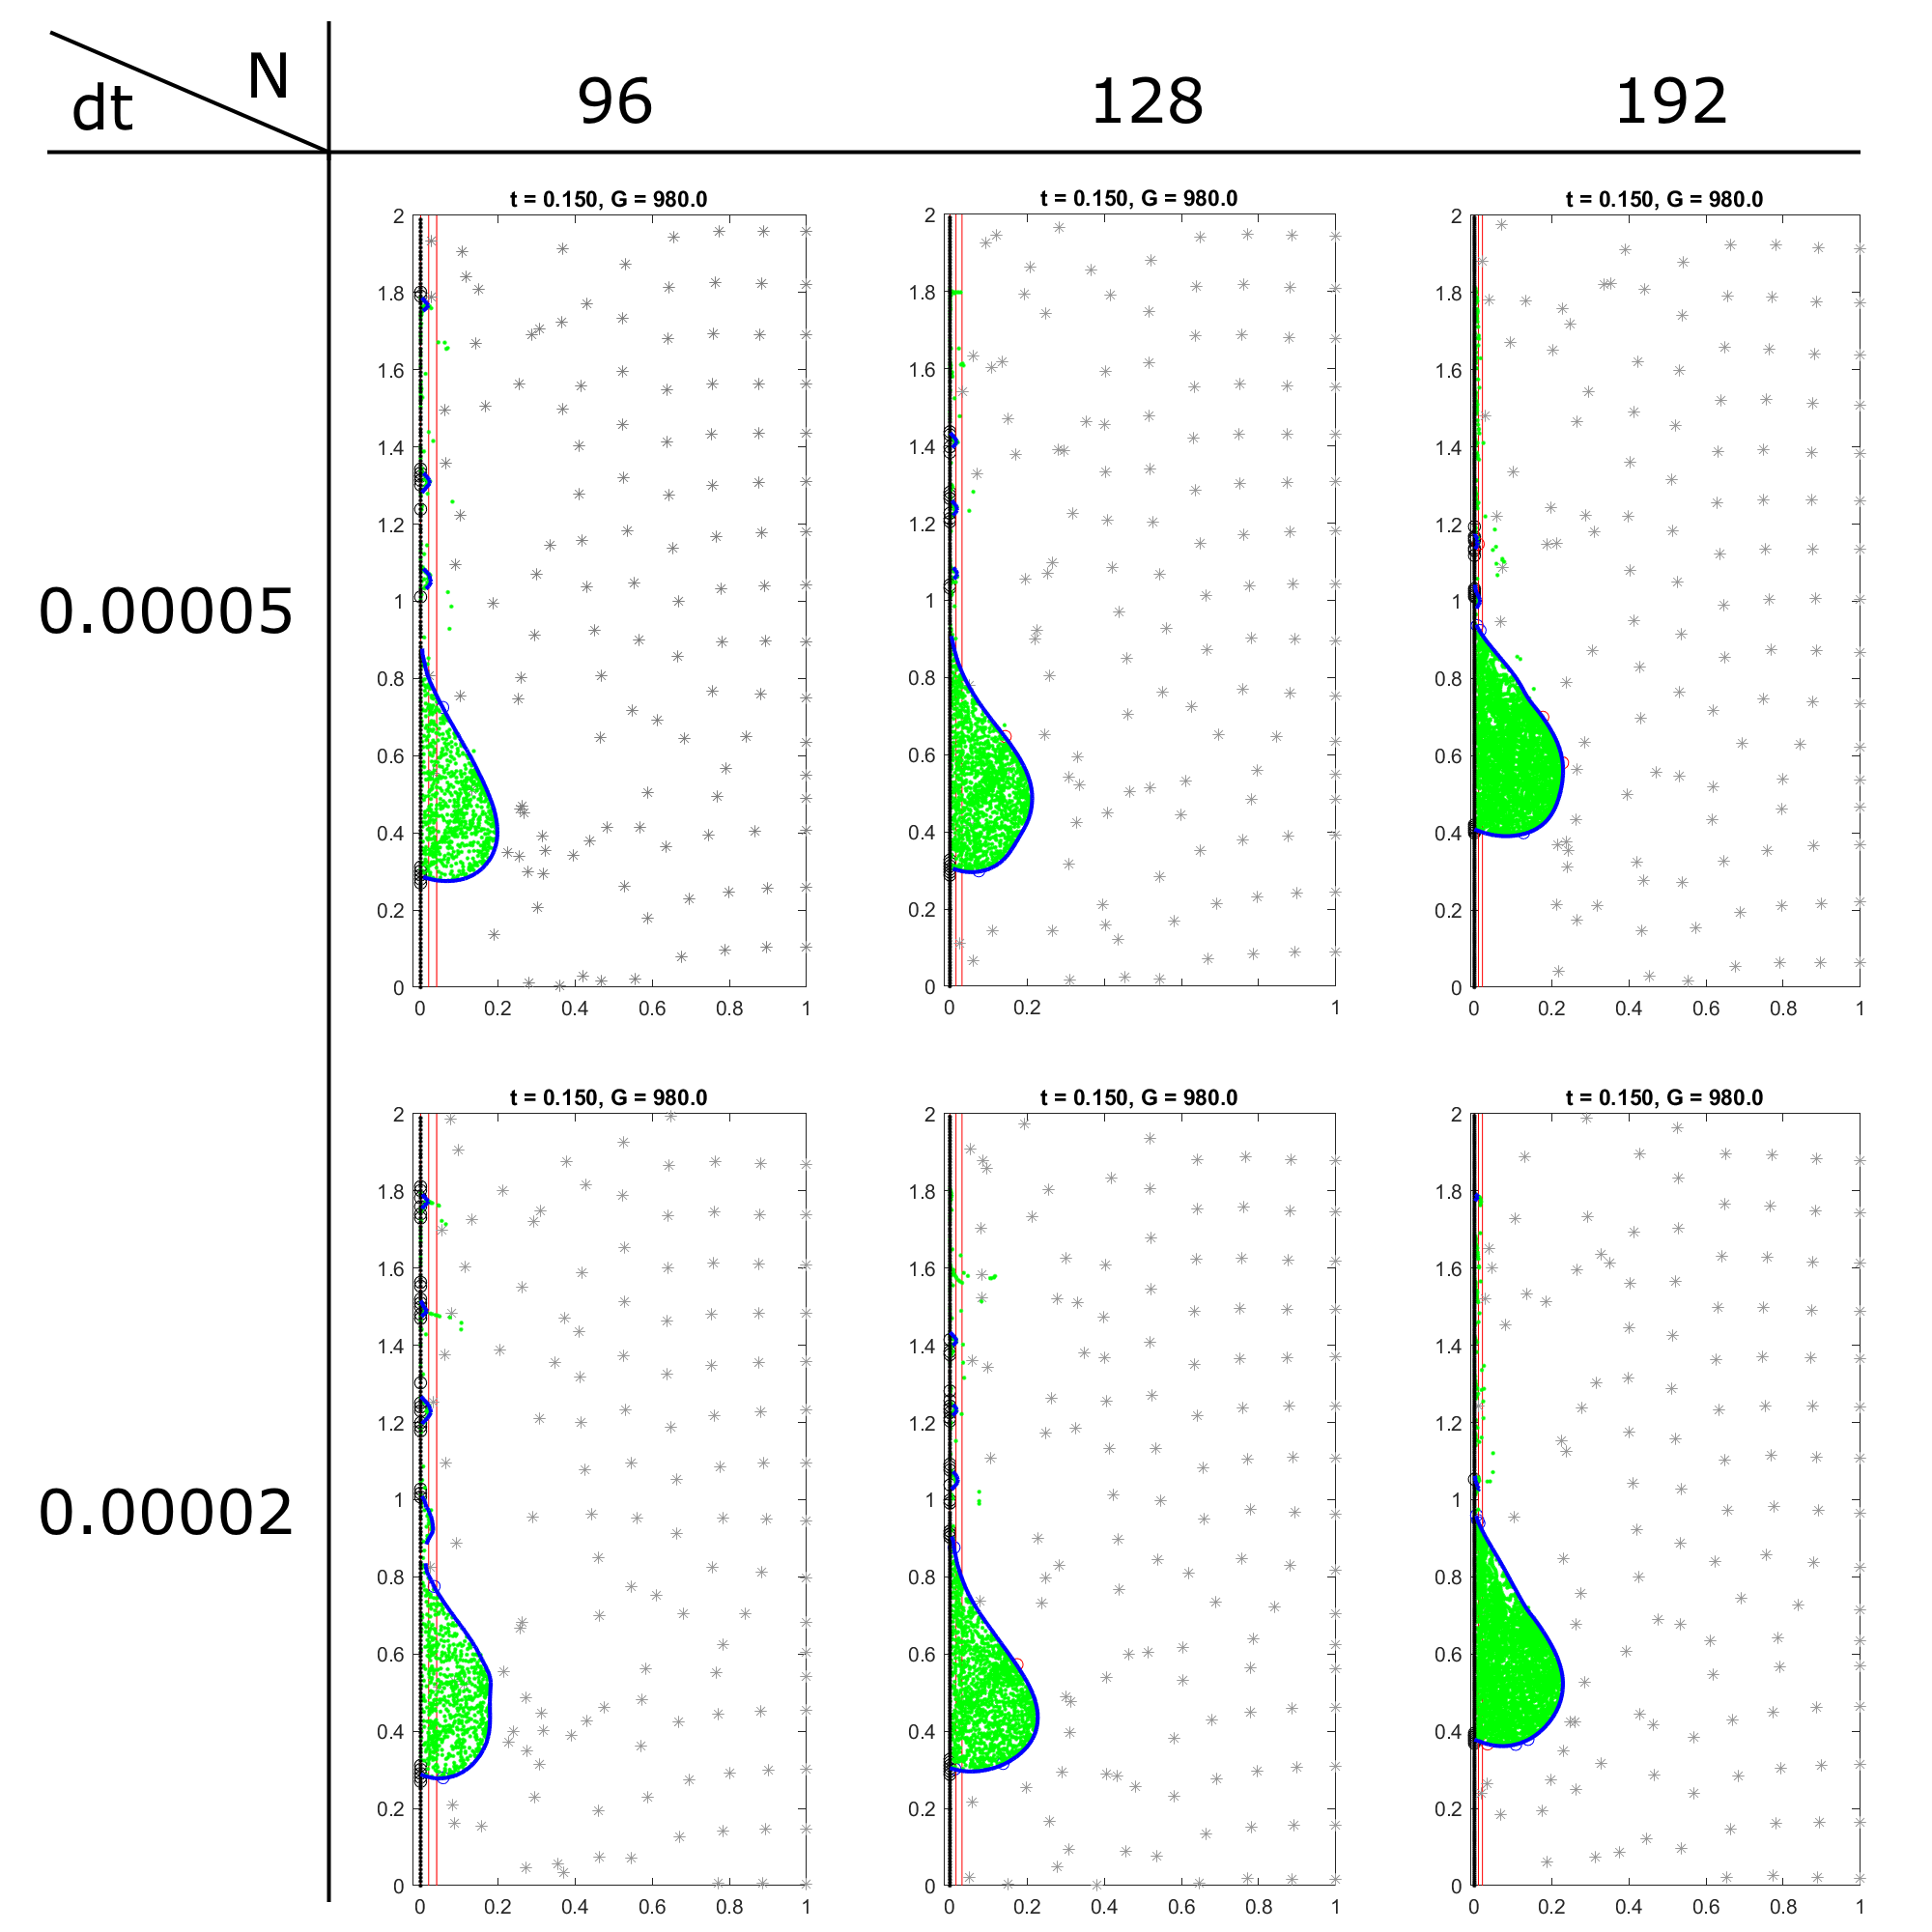
\includegraphics[scale=0.6]{figs/terminal.pdf} 
\caption{Terminal state of the sliding droplet simulation for several different values of $dt$ and $N$. The axes units are in cm. The simulation is terminated after the droplet stops moving. Notice the trail of fluid left by the droplet as it slides down the wall. Further increasing $N$ beyong $192$ yields no visible changes in the results.}
\label{fig:terminal}
\end{figure}
We simulate a droplet sliding down a vertical wall as shown in figure ~\ref{fig:terminal}.  Details can be found in subsection \ref{subsec:dow}. In this case, gravity competes with sliding friction and upward airflow. We vary the time step $dt$ and the spatial discretization resolution $N$, and we depict the terminal state ($t = 0.15$ s). We observe that improvement is achieved if we increase the spatial discretization resolution $N$ to $192$. Further increasing $N$ beyond this value yields no visible improvement. See movie 4 for the simulation video.

\subsubsection {Test 2: Coalescence of two droplets}
In this test case, the height of the computational domain is $L=2$ cm, the tension coefficient is $\sigma=50$ g\,cm/s$^2$, the gas density is $\rho_g=0.1$ g/cm$^2$, the liquid density is $\rho_l=1$ g/cm$^2$, and the viscosity is $\mu=0.01$ g/s. 
\begin{figure}
\centering
\begin{lapsetable}{6}{.12}
$N$ & $dt$ & $t$=0.01 s&0.02 s&0.03 s&0.04 s&0.05 s&0.06 s
\lapse{merge2}{0.000500}{64} {\scinote{5}{-4}}{6}{5.5}{4}{4.8}{1.5}
\lapse{merge2}{0.000200}{96} {\scinote{2}{-4}}{6}{5.5}{4}{4.8}{1.5}
\lapse{merge2}{0.000100}{128}{\scinote{1}{-4}}{6}{5.5}{4}{4.8}{1.5}
\end{lapsetable}
\caption{This figure shows the coalescence of two droplets. Three levels of spatial and temporal resolutions are shown. Little improvement is gained from $N = 96$ to $N = 128$, rendering $N = 128$ a high enough spatial resolution (holding other parameters constant).}
\label{fig:merge_two}
\end{figure}
In this section, we simulate two droplets coalescing as shown in figure ~\ref{fig:merge_two}. The coalescence of two droplets is an extremely challenging test case since the moment of droplet merging amplifies previous numerical perturbations. The simulation results show good spatial and temporal convergence with our surface tension model and interface splicing techniques. See movie 5 for the simulation video.

\subsubsection {Test 3: Coalescence of six droplets}
In this test case, the height of the computational domain is $L=2$ cm, the tension coefficient is $\sigma=50$ g\,cm/s$^2$, the gas density is $\rho_g=0.1$ g/cm$^2$, the liquid density is $\rho_l=1$ g/cm$^2$, and the viscosity is $\mu=0.01$ g/s. 

\begin{figure}
\centering
\begin{lapsetable}{6}{.13}
$N$ & $dt$ & $t$=0.01 s&0.02 s&0.03 s&0.04 s&0.05 s&0.06 s
\lapse{merge6}{0.000200}{96} {\scinote{2}{-4}}{6}{3.4}{3.8}{2.3}{1.5}
\lapse{merge6}{0.000100}{128}{\scinote{1}{-4}}{6}{3.4}{3.8}{2.3}{1.5}
\lapse{merge6}{0.000050}{192}{\scinote{5}{-5}}{6}{3.4}{3.8}{2.3}{1.5}
\end{lapsetable}
\caption{Six droplets coalesce under three levels of spatial and temporal resolutions. Little improvement is gained from $N = 128$ to $N = 192$, rendering $N = 192$ a high enough spatial resolution (holding other parameters constant).}
\label{fig:merge_six}
\end{figure}
In this section, we simulate six droplets coalescing as shown in figure ~\ref{fig:merge_six}. The six-droplet merging test is even more challenging, since the variance of the system's response to the first coalescence event is amplified by the successive merging events. Our system demonstrates an interesting property that large values of $dt$ lead to instability issues, and slowly lowering $dt$ into a stable regime leads to fast convergence and high accuracy. See movie 6 for the simulation video.

\subsubsection {Test 4: Letters "IB" fall into an elastic pouch}
\label{subsubsec:letters}
In this test case, the height of the computational domain is $L=10$ cm, the tension coefficient is $\sigma=50$ g\,cm/s$^2$, the gas density is $\rho_g=0.1$ g/cm$^2$, the liquid density is $\rho_l=1$ g/cm$^2$, and the viscosity is $\mu=0.01$ g/s. 

\begin{figure}
\centering
\begin{lapsetable}{7}{.12}
$N$ & $dt$ & $t$=0 s&0.03 s&0.06 s&0.09 s&0.12 s&0.15 s&0.24 s
\lapse{letters}{0.0005}{96} {\scinote{5}{-4}}{7}{6}{4}{5}{5}
\lapse{letters}{0.0003}{128}{\scinote{3}{-4}}{7}{6}{4}{5}{5}
\end{lapsetable}
\caption{Letter-shaped droplets falling into elastic pouch, simulated with two levels of spatial and temporal resolutions. This demos our method's capability for simulating MCL on a changing-shape solid surface. }
\label{fig:letters}
\end{figure}
Here we initialize liquid droplets in the shape of Latin letters ``IB" and let them fall into an elastic pouch (figure ~\ref{fig:letters}). At the beginning of the simulation, the droplets change shape under surface tension, eliminating sharp corners. As the droplets hit the pouch, the pouch deforms and the gas bubbles make their way out from the liquid body. This test case demonstrates the capabilities of our method in an all-in-one setting. Note that here the solid membrane is dynamic, rendering static boundary conditions unusable. This shows that our methods are capable of simulating a moving contact line between a liquid-gas interface and a changing-shape solid surface, simulating fluid dynamics, surface tension, unbalanced Young stress, extended GNBC, and solid elasticity at the same time. See movie 7 for the simulation video.

\charles{cool, so you are using GNBC on the elastic pouch??????} \daniel{yes. extended GNBC}

\subsection {Performance of the re-sampling technique \charles{put in appendix?}} \label{subsec:resample}
\begin{figure}
\centering
\begin{shortlapsetable}{3}{.23}
Re-sample & $t$=0.028 s&0.045 s&0.078 s
\tabularnewline Off
\lapseShort{resample/bad}{3}{7}{4}{8.5}{5}
\tabularnewline On
\lapseShort{resample/good}{3}{7}{4}{8.5}{5}
\end{shortlapsetable}
\caption{As fluid flow advects the interface markers, if the re-sampling step is turned off, then the interface breaks into pieces and the holes start to allow penetration.}
\label{fig:resample_comp}
\end{figure}
figure ~\ref{fig:resample_comp} shows a comparison study on the effect of our step-wise re-sampling technique. In the upper row, we do not re-sample, resulting in badly distributed Lagrangian markers and, eventually, topological errors. On the lower row, adding the re-sampling technique fixes the problem. See movie 8 for the simulation video.

\subsection {Demos of interface splicing \charles{put in appendix?}} \label{subsec:more_splice}
\begin{figure}
\centering
\begin{shortlapsetable}{7}{.13}
$t$=&0.187 s&0.190 s&0.193 s&0.197 s&0.2 s&0.103 s&0.207 s
\tabularnewline
\lapseShort{split}{7}{6.4}{4.2}{4.6}{4.8}
\end{shortlapsetable}
\caption{A droplet splits into two.}
\label{fig:split}
\end{figure}
    
\begin{figure}
\centering
\begin{shortlapsetable}{8}{.09}
$t$=&0.019 s&0.021 s&0.022 s&0.024 s&0.027 s&0.029 s&0.035 s&0.040 s
\tabularnewline
\lapseShort{wall_merge}{8}{5}{4.8}{9.5}{3.5}
\end{shortlapsetable}
\caption{Two droplets merge on the wall.}
\label{fig:wall_merge}
\end{figure}
In figure ~\ref{fig:split}, a droplet separates into two smaller ones. After the splicing moment, surface tension quickly brings the sharp edge into the body of the droplet. In figure ~\ref{fig:wall_merge}, two droplets coalesce on the wall. This is one of the six basic cases of interface splicing. Additional simulations can be found in movie 9 through 13. 
    
% \subsection {Energy and Area Conservation}
%     \daniel{I can track the energy error from interface re-sampling and splicing.}
%     \daniel{Do it!}
%     \daniel{But I did not keep the plotting script QAQ}

% \subsection {Spurious Currents}
%     [compare shrink]
%     \daniel{Do we even include this part? I think Puelz once said this is just well-known for IB methods.}

% \subsection {Computation Costs and Instability Issues}
%     \begin{figure}
%         \begin{subfigure}{.5\textwidth}
%         \centering
%         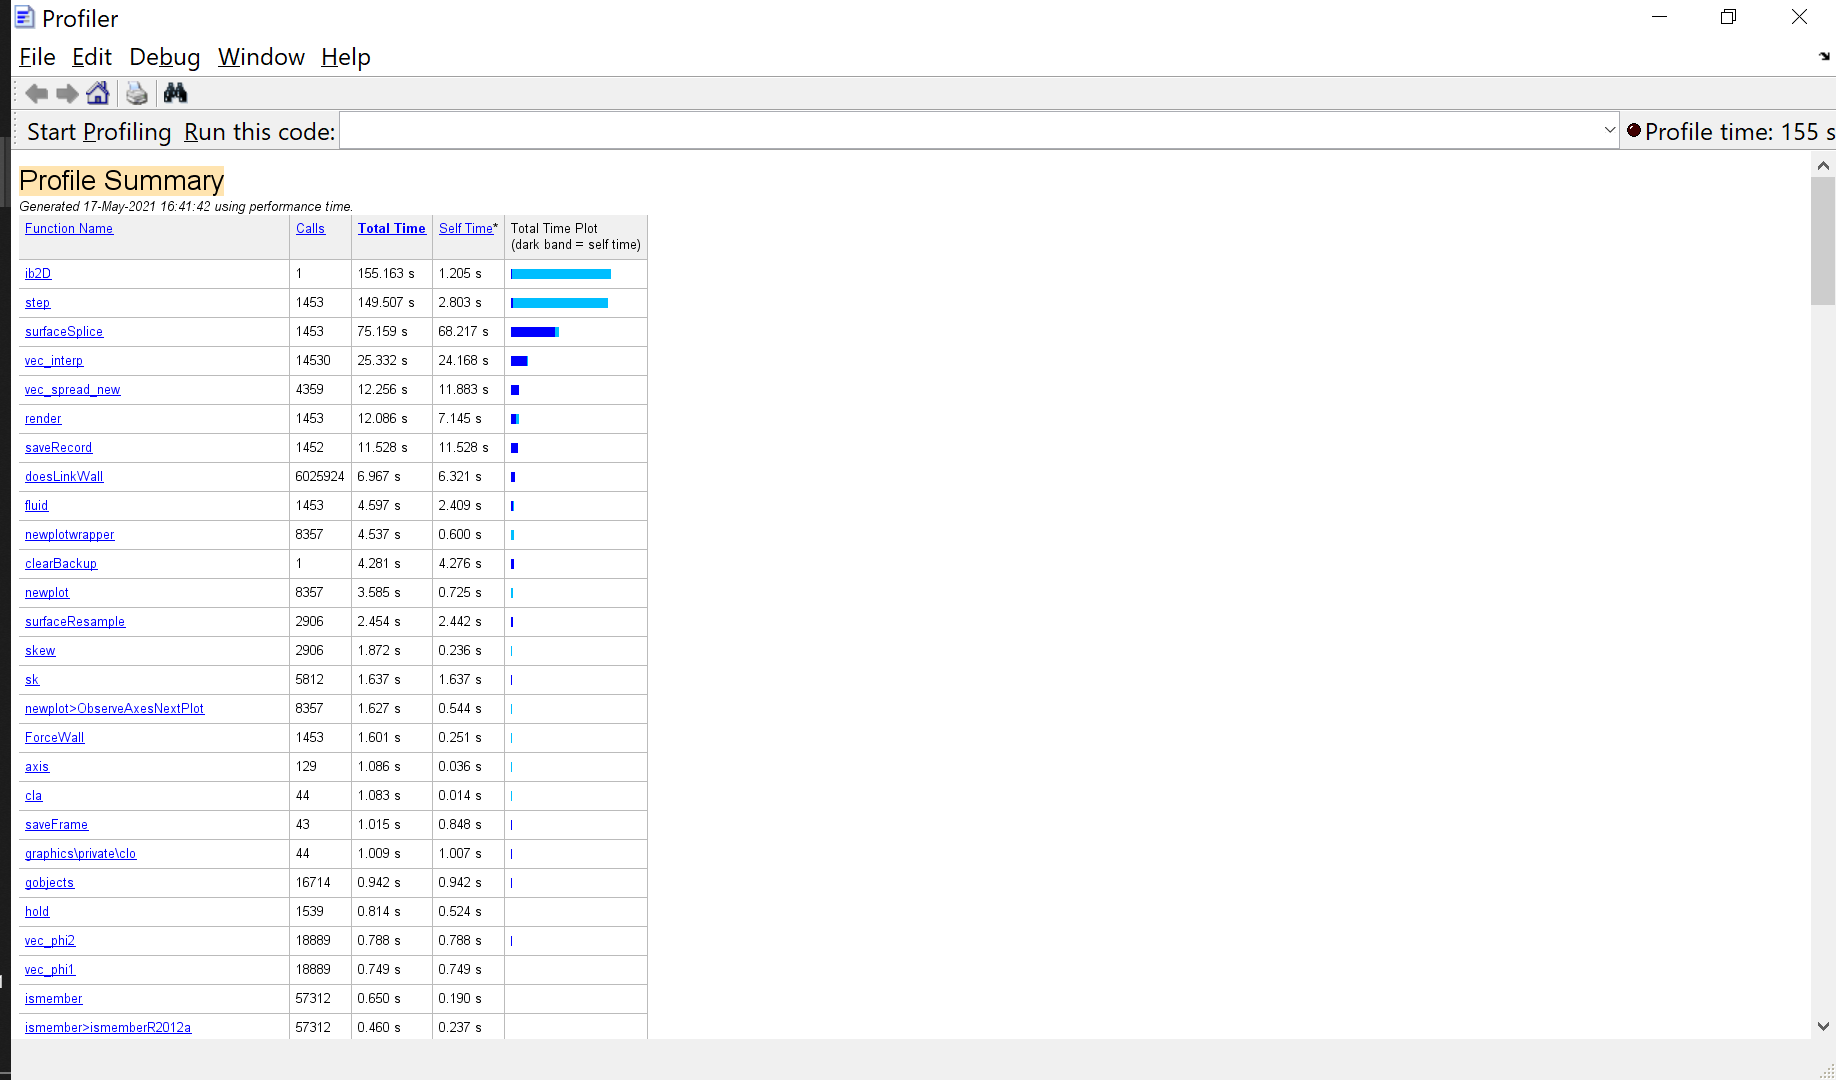
\includegraphics[width=\textwidth,trim={0mm 0mm 0mm 0mm},clip]{figs/time_profiling/summary.pdf}
%         \end{subfigure}
%         \begin{subfigure}{.5\textwidth}
%         \centering
%         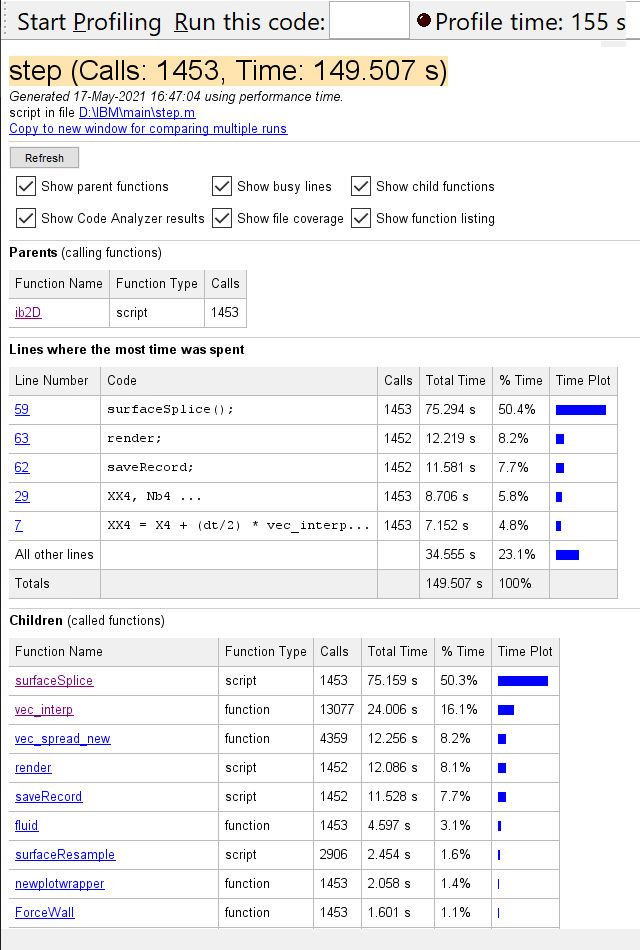
\includegraphics[width=\textwidth,trim={0mm 0mm 0mm 0mm},clip]{figs/time_profiling/step.pdf}
%         \end{subfigure}
%         \\
%         \begin{subfigure}{.36\textwidth}
%         \centering
%         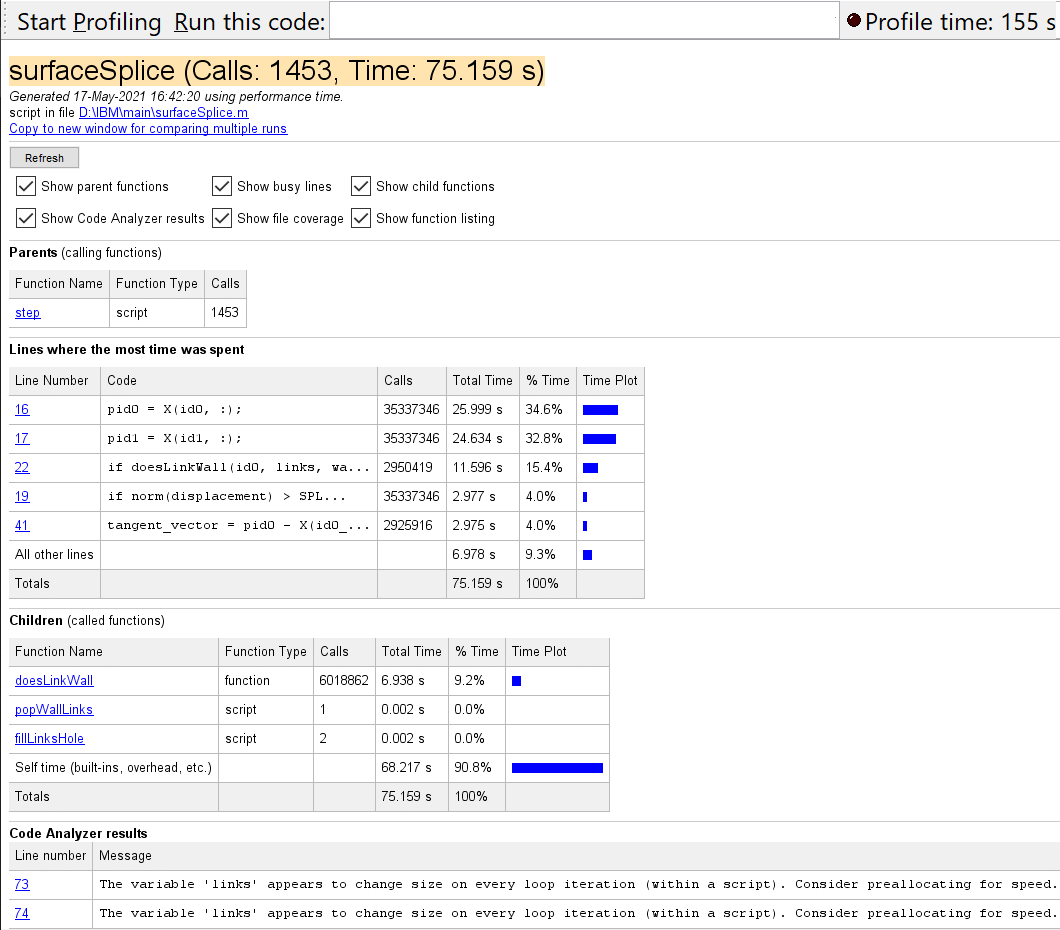
\includegraphics[width=8cm,trim={0mm 0mm 0mm 0mm},clip]{figs/time_profiling/surfaceSplice.pdf}
%         \end{subfigure}
%         \begin{subfigure}{.64\textwidth}
%         \centering
%         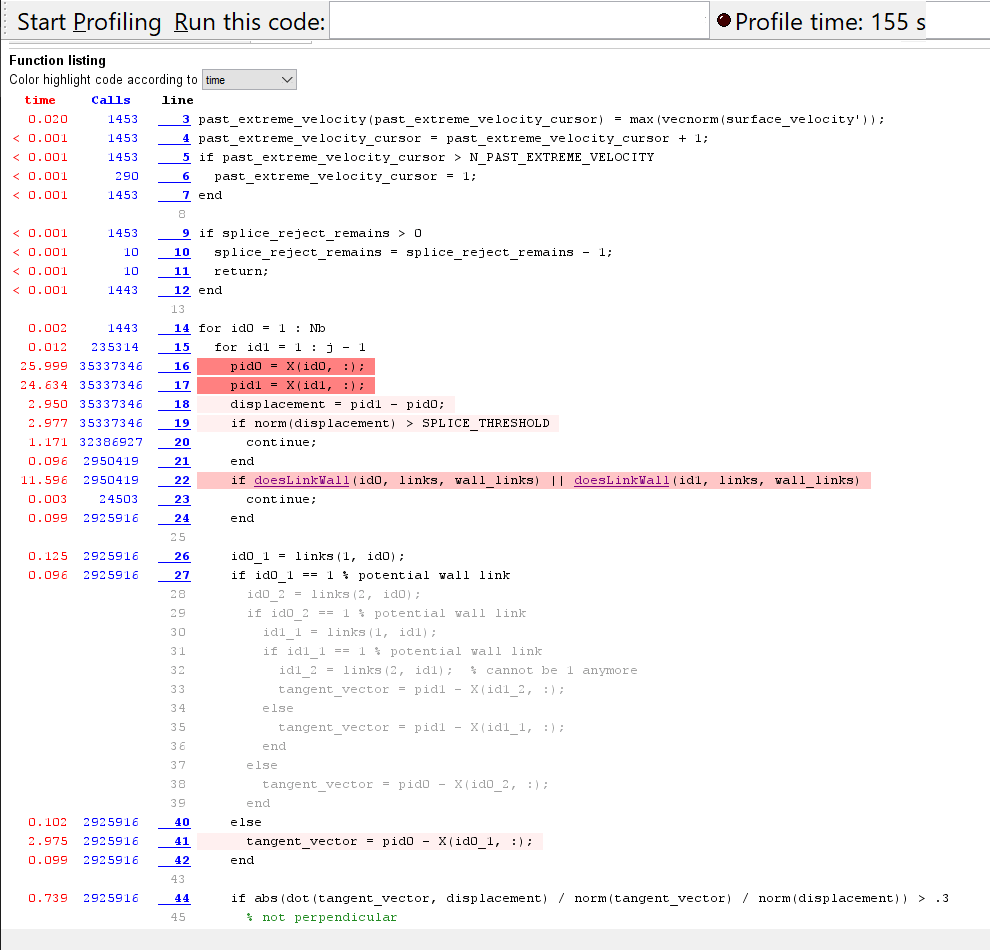
\includegraphics[width=\textwidth,trim={0mm 0mm 0mm 0mm},clip]{figs/time_profiling/code.pdf}
%         \end{subfigure}
%         \caption{
%             Matlab profiler showing the time consumption at each step of the simulation. Interface splicing is the most expensive computation. 
%         }
%         \label{fig:computation}
%     \end{figure}

%     Figure \ref{fig:computation} shows the time consumption of various computations involved in our method. The most expensive computation out of the box is interface splicing. This is due to its $O(N^2)$ nature. Despite the optimization tricks mentioned in \ref{subsec:splice}, it is still the main cost of simulation. The second slowest operation is the vector interpolation for the variable density \citep{kim2008numerical} markers. Spreading the 2D soup of markers to the Eulerian grid is expensive. The rest of the operations are in the same timescale with the vanilla IB method. 
    
%     The existence of surface tension poses a stiffness problem. $dt$ has to be very small to avoid instability. We also observe that, the finer the spatial resolution, the smaller the time step needs to be. Otherwise, spurious oscillating fluid velocity will emerge and quickly drives everything to NaN. 
    
%     The interface re-sampling algorithm makes a minor contribution to the instability. This is intuitive in a sense that removing a marker forces a previously-curving surface to become straight. Although the effect is minimal, it does apply a spurious normal force to the fluid interface. This then encourage theadjacent markers to bend in the other direction, forming a zigzag pattern. In reality, this issue only occurs very rarely. 

\section{Conclusions} \label{sec:conclusion}
We propose and test four techniques that work with the immersed boundary method. An extended GNBC wall can be modeled as an immersed boundary and the friction forces are directly spread at the wall. The surface tension and the unbalanced Young force can be nicely integrated under IB by computing local unit vectors tangent to the interface. We also show that interface marker re-sampling is necessary for correct results. Our interface splicing method handles droplet coalescence, separation and other topological changes with stable splicing events. 

Our work is limited in several ways. Our methods always assume the fluids to be incompressible. We expect the interface splicing method to be the most vulnerable to a compressible-flow setting. Inertia and compressibility will be likely to make the splicing events much less atomic. In addition, although our methods support variable density, it does not support variable viscosity. They only deal with multiple fluid phases of 1:1 viscosity ratio. 

The success of our methods demonstrates the rich extensibility of the IB method. We have showed that even complex dynamics such as the moving contact line on an evolving solid surface can be modeled with the IB method. 

Additionally, many equivalent ways of modelling the same phenomena can converge to the same results. For example, among many possible ways of implementing the wall friction, we choose to displace wall markers so that the tether force density equals the friction density, and the baseline IB method imparts the tether force onto the fluid. There are many other ways to do the same thing: for example, formulating the friction as an additional type of force, directly imparting the friction onto the fluid without intermediate markers, or prescribing the fluid velocity according to local tangential stress. What we proposed may not be the most efficient, so further testing is welcome. 
\daniel{I don't know, drop the last paragraph?}

\backsection[Supplementary data]{\label{SupMat}Supplementary movies are submitted with the paper as movie 1 through 15. }

\backsection[Acknowledgements]{We thank Otto Mierka and Stefan Turek for providing the 10:10 viscosity benchmark data for rising bubble test case 1. Several very helpful conversations with Guanhua Sun are gratefully acknowledged.}

\backsection[Funding]{P.S. is supported by an Institutional Support of Research and Creativity (ISRC) grant provided by New York Institute of Technology and financial support from the National Science Foundation (NSF) under Grants No. DMS-2108161.}
\daniel{Please provide details of the sources of financial support for all authors, including grant numbers. For example, "This work was supported by the National Science Foundation (grant number XXXXXXX)". Multiple grant numbers should be separated by a comma and space, and where research was funded by more than one agency the different agencies should be separated by a semi-colon, with 'and' before the final funder. Grants held by different authors should be identified as belonging to individual authors by the authors' initials. For example, "This work was supported by the Deutsche Forschungsgemeinschaft (A.B., grant numbers XXXX, YYYY), (C.D., grant number ZZZZ); the Natural Environment Research Council (E.F., grant number FFFF); and the Australian Research Council (A.B., grant number GGGG), (E.F., grant number HHHH)". \\
Where no specific funding has been provided for research, please provide the following statement: "This research received no specific grant from any funding agency, commercial or not-for-profit sectors."}

\backsection[Declaration of interests]{A {\bf Declaration of interests} statement is now mandatory in the manuscript PDF. Please included a statement in your manuscript at the end of the main text with regards to any known competing financial interests or personal relationships that could appear to have influenced the work reported in this paper. These must also be declared in your covering letter to the Editor. Please note that if there are no conflicts of interest, the declaration in your PDF should read as follows: {\bf Declaration of Interests}. The authors report no conflict of interest.}

\backsection[Data availability statement]{
All simulations in this study can be reproduced with the source code openly available at repository https://github.com/daniel-chin/droplet. The repository also contains the scripts to plot all the figures. 
}

\section{Appendices} 
\subsection{Analytical modelling of the hanging droplet equilibrium} \label{app:equi}
    The shape of the hanging droplet is determined by the following equations:\\
    \begin{equation}
        \vec{g}=g\cdot\hat{j}, \quad
        \nabla{p}=\rho\cdot{g}, \quad
        \frac{\mathrm{d}p}{\mathrm{d}y}=-\rho\cdot{g}, \quad
        p=-\rho\cdot{g}\cdot{y}+p_{\text{const.}}
    \end{equation}
    At the interface, we define the surface tension as:\\
    \begin{equation}
        p=p_{a}+\sigma \cdot \kappa(s),
        \label{eq:pressure}
    \end{equation}
    where $p_{a}$ is the air pressure, and $\kappa(s)$ is the surface curvature. By parametrization of the surface, we get:\\
    \begin{align}
        r(s)=x(s)\cdot\hat{i}&+y(s)\cdot\hat{j}.\\
        \hat{t}=\frac{\mathrm{d}r}{\mathrm{d}s}=x(s)'\cdot\hat{i}&+y(s)'\cdot\hat{j}.
    \end{align}
    We normalize the derivative by writing $1=\left(\frac{\mathrm{d}x}{\mathrm{d}s}\right)^2+\left(\frac{\mathrm{d}y}{\mathrm{d}s}\right)^2$. We get $\left|\frac{\mathrm{d}x}{\mathrm{d}s}\right|=\sqrt{(x')^2+(y')^2}=1$\\
    We define the normal vector as\\
    \begin{center}
        $\hat{n}=\hat{t}\times\hat{k}=y'(s)\hat{i}-x'(s)\hat{j}$.
    \end{center}
    Now we have a system of ODEs:\\
    \begin{equation}
        \frac{\mathrm{d}\hat{t}}{\mathrm{d}s}=-x\hat{n}(s), \quad
        \frac{\mathrm{d}\hat{n}}{\mathrm{d}s}=x\hat{t}.
    \end{equation}
    By some algebra, we get\\
    \begin{center}
        $x''(s)\hat{i}+y''\hat{j}=-x\hat{n}$.
    \end{center}
    Multiply both sides by $\hat{n}$, we get\\
    \begin{equation}
        -x=y'x''-x'y''. 
        \label{eq:curvature}
    \end{equation}
    The above equation is the curvature expression for our reparametrization.\\
    Plug \ref{eq:curvature} into \ref{eq:pressure}, we get\\
    \begin{align}
        p-\rho\cdot{g}\cdot{y(s)}&=p_{a}+\sigma(x'y''-y'x'')\\
        x'y''-y'x''+\frac{\rho\cdot{g}}{\sigma}y&=\frac{\Delta{p}}{\sigma}.
    \end{align}
    Define the capillary length $l=\sqrt{\frac{\sigma}{\rho\cdot{g}}}$,
    and by rescaling, we get\\
    \begin{center}
        $x'y''-y'x''+\frac{u}{l^2}=\frac{\Delta{p}}{\sigma}$.
    \end{center}
    Rescaling $x$, $y$ and $s$ in terms of $l$, we get\\
    \begin{center}
        $\bar{x}=\frac{x}{l}$, \quad $\bar{y}=\frac{y}{l}$, \quad $\bar{s}=\frac{s}{l}$, \quad $\Pi=\frac{l\Delta P}{\sigma}$.
    \end{center}
    We rewrite the equation in dimensionless form\\
    \begin{equation}
        x'y''-y'x''+y=\Pi.
    \end{equation}
    Without loss of generality, set initial conditions $x(0)=y(0)=0$. The first order initial conditions can be described by the contact angle $\theta$: 
    \begin{equation}
        \begin{cases}
            x'(0)=\sin(\theta)\\
            y'(0)=\cos(\theta).
        \end{cases}
    \end{equation}
    
    The above model describes the hydro-static equilibrium shape of a droplet hanging on a vertical wall as a PDE in the Cartesian space. The result shows that there is a linear relationship between the local curvature of the interface and the altitude. 

\bibliographystyle{jfm}
\bibliography{mybibfile}
% \begin{thebibliography}{99}

% \bibitem[Sanaei {\it et al.}(2016)]{Sanaei2016}
% {\sc Sanaei, P., Richardson, G.W., Witelski, T., Cummings, L.J.,}
% Flow and Fouling in a Pleated Membrane Filter.
% {\it J. Fluid Mechanics.} {\bf 795}, 36-59 (2016).

% \bibitem[Sanaei {\it et al.}(2017)]{Sanaei2017}
% {\sc Sanaei, P., Cummings, L.J.,}
% Flow and fouling in membrane filters: Effects of membrane morphology.
% {\it published at J. Fluid Mechanics.} (2017)

% %\bibitem[Sanaei {\it et al.}(2017)]{Sanaei2017cake}
% %{\sc Sanaei, P., Cummings, L.J.,}
% %Optimum Permeability Profile and Fouling in Membrane Filters.
% %{\it Preprint.}

% \end{thebibliography}

\end{document}             % End of document.
